\chapter{Los Ratios Financieros}
Los ínfices o ratios entre distintos datos del Balance y otras cuentas de los estados financieros, permiten efectuar un rápido análisis financiero de la empresa. Son particularmente útiles para:
\begin{itemize}
    \item Hacer comparaciones entre empresas del mismo sector
    \item Comprender la política que sigue un competidor
    \item Conocer la solidez financiera de un potencial cliente
    \item Analizar la situación financiera de la propia empresa y posibilidades de mejora
\end{itemize}

Diferentes clases de ratios financieros:
\begin{itemize}
    \item Ratios de Liquidez, miden la facilidad con la que una empresa puede conseguir tesorería.
    \item Ratios de Endeudamiento, miden el nivel de endeudamiento de la empresa.
    \item Ratios de Eficiencia o Rotación, miden la productividad con que la empresa emplea sus activos.
    \item Ratios de Rentabilidad, miden la rentabilidad sobre inversiones actuales de una empresa.
\end{itemize}

\section{Ratios de Rentabilidad: Márgenes ROA ROE}
Miden la capacidad de generación de beneficio por parte de la empresa. Tienen por objetivo evaluar los resultados económicos de la actividad empresarial valorando el resultado neto obtenido a partir de ciertas decisiones y políticas en la administración de los fondos de la empresa.

Expresan el rendimiento de la empresa en relación con sus ventas, activos o capital. Relacionan directamente la capacidad de generar fondos en operaciones de corto plazo.

Miden la eficiencia con la que la emrpesa gestiona los recursos que han aportado los proveedores de fondos, i.e, accionistas y acreedores.

Su numerador contiene alguna definición particular del beneficio, mientras que su denominador presenta inversiones de distinta naturaleza efectuadas por la empresa.

La estabilidad de los beneficios es siempre un atractivo para el inversor, así ratios de rentabilidad estables, indican capacidad de adaptación al entorno.

\section{Los márgenes del negocio}
Los márgenes aportan información de la `calidad' del beneficio:
\begin{itemize}
    \item tiene un buen nibel,
    \item Se mantiene en el tiempo, es decir, está basado fundamentalmente en operaciones de explotación
\end{itemize}

Para su interpretación hay que tener en cuenta el sector en el que opera la empresa.

\[ Margen\ de\ Explotacion = \frac{BAII}{Ventas}\ o\  \frac{EBIT}{Ventas}\]
\[Margen\ Operativo = \frac{BAI}{Ventas}\]
\[Margen\ Neto = \frac{BN}{Ventas}\]

\section{Ratios de Rentabilidad ROA-ROE-ROIC}
\[ROA = \frac{BAII}{Activo\ Total}\]
\[ROE = \frac{BN}{Fondos\ propios}\]
\[ROIC = \frac{BAII*(1-T)}{Fondos\ propios + deuda}\]

Permiten efectuar un rápido análisis financiero de la empresa. Muy útiles a nivel comparativo entre empresas del mismo sector.

\section{Relación entre ROA-ROE}
La relación entre el ROE, el ROA y el apalancamiento en la siguiente ecuación:
\[ROE = ( ROA + (ROA - Tasa\ de\ Interes)(\frac{P}{FP}))*(1 - Tasa\ Impositiva)\]
El ROE dependerá así de cuatro factores:
\begin{itemize}
    \item la eficiencia vía margen de beneficio
    \item la rotación según el uso de los activos
    \item el apalancamiento financiero y 
    \item el efecto fiscal
\end{itemize}

\section{Diferencias ROA ROE}
La principal diferencia (denominador)
\begin{itemize}
    \item En la rentabilidad financiera se tienen en cuenta los fondos propios que tiene la empresa para la obtención de beneficios.
    \item En la rentabilidad económica se tiene en cuenta el activo total de la empresa para conocer los beneficios obtenidos.
\end{itemize}

Otra diferencia entre rentabilidad económica y financiera es el beneficio que se utiliza para calcularlas (numerador):
\begin{itemize}
    \item La rentabilidad financiera relaciona el beneficio una vez deducidos los intereses, impuestos y posibles gastos financieros.
    \item La tentabilidad económica relaciona el beneficio antes de intereses e impuestos, sin tener en cuenta los gastos financieros que han supuesto la financiación de los activos totales de la empresa.
\end{itemize}

Por último y no menos importante, una de las diferecncias entre rentabilidad económica y financiera es el denominado Apalancamiento.

\section{¿Qué es el apalancamiento?}
El apalancamiento, también denominado ``Efecto palanca'' consiste en financiarse mediante recursos ajenos (endeudamiento) para recuperar determinadas inversiones que se han realizado en la empresa.

Se puede decir una empresa está apalancada cuando aumenta su pasivo (sus deudas) para adquirir activos.

\section{Apalancamiento. La relación entre ROA-ROE}
\paragraph{Apalancamiento Positivo: El ROE > ROA.} Esto significa que el coste medio de las deudas de la empresa es inferior a la rentabilidad económica que obtiene. Por tanto, financiar parte del activo con recursos ajenos ha hecho aumentar la rentabilidad financiera.

\paragraph{Apalancamiento Negativo: El ROE < ROA.} El coste medio de las deudas de la empresa para financiar sus activos supera a la rentabilidad económica.

\paragraph{Apalancamiento Nulo: El ROE = ROA.} Este tipo de apalancamiento se da en los casos en que el activo de la empresa se financia con fondos propios, sin recurrir a la financiación externa.

\section*{Retorno sobre el Capital Invertido ROIC}
Cuantifica la rentabilidad que han obtenido los inversionistas (accionistas y acreedores) por el capital aportado para financiar los proyectos de inversión de la empresa.
\[ ROIC = EBIT \times \frac{1 - Tasa\ impositiva}{Fondos\ propios + Deuda\ con\ coste}\]

El ROIC depende así de dos factores:
\begin{itemize}
    \item la eficiencia vía margen operativo y
    \item el coste fiscal
\end{itemize}

\[NOPAT = EBIT \times (1 - Tasa\ impositiva)\]

NOPAT (Beneficio operativo después de impuestos). Mide la rentabilidad que obtiene cada euro que la empresa ha invertido en su propio negocio y debe ser comparado con el coste de sus fuentes de financiación.

\section*{Efecto del endeudamiento}
Pero para esto sea cierto, tenemos que suponer que:
\begin{enumerate}
    \item Las decisiones de financiación no afectan a la rentabilidad ni al riesgo de las operaciones de la empresa; en consecuencia, la rentabilidad de los activos ($R_{AN} = BAIT \times \frac{1 - t}{Activo\ total}$), permanece inalterada cualquiera que sea estructura de financiación, y
    \item con la nueva deuda incurrida se recomprarán acciones.
\end{enumerate}

Puesto que la $R_{AN}$ permanece constante, el beneficio después de impuestos en realidad disminuye cuando aparece la deuda, resulta que cuando se dice que el endeudamiento puede tener un impacto favorable en los resultados se hace referencia a resultados que tienen que ver con los accionistas: $BPA$ y $R_{RP}$. En una óptica contable, estas variables son el punto de referencia para la evaluación del endeudamiento.

\begin{figure}[h]
    \centering
    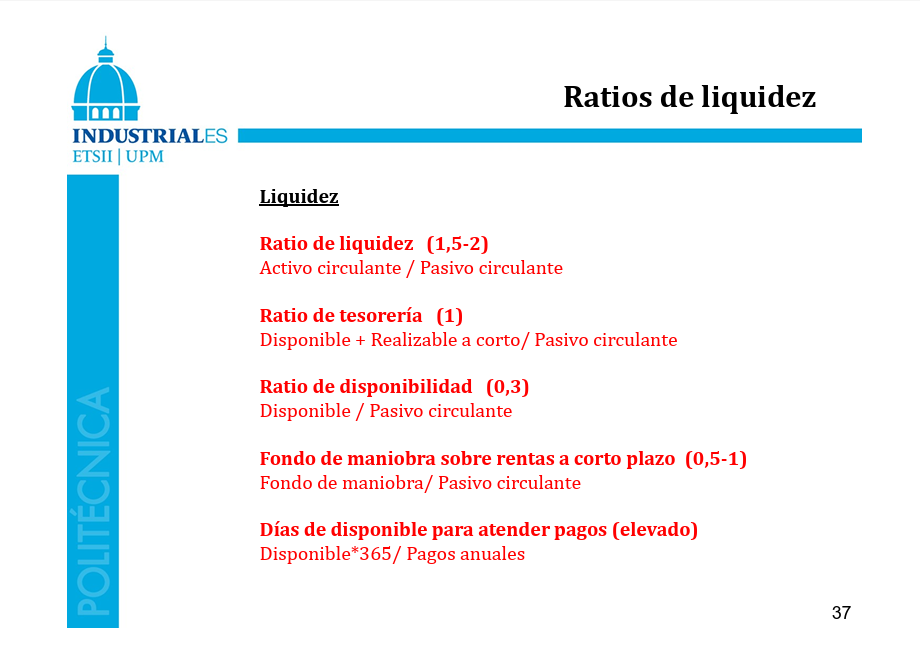
\includegraphics[width = \linewidth]{Imagenes/Ratios de liquidez.png}
    \caption{Ratios de liquidez}
    \label{fig:ratios de liquidez}
\end{figure}

\begin{figure}[h]
    \centering
    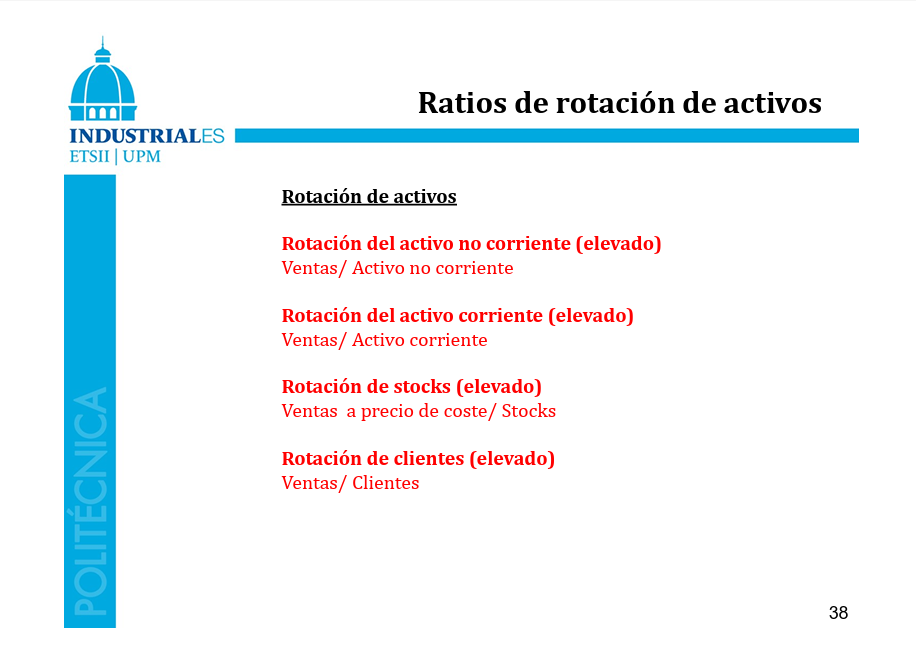
\includegraphics[width = \linewidth]{Imagenes/Ratios de rotacion de activos.png}
    \caption{Ratios de rotación de activos}
    \label{fig:ratios de rotacion de activos}
\end{figure}

\begin{figure}[h]
    \centering
    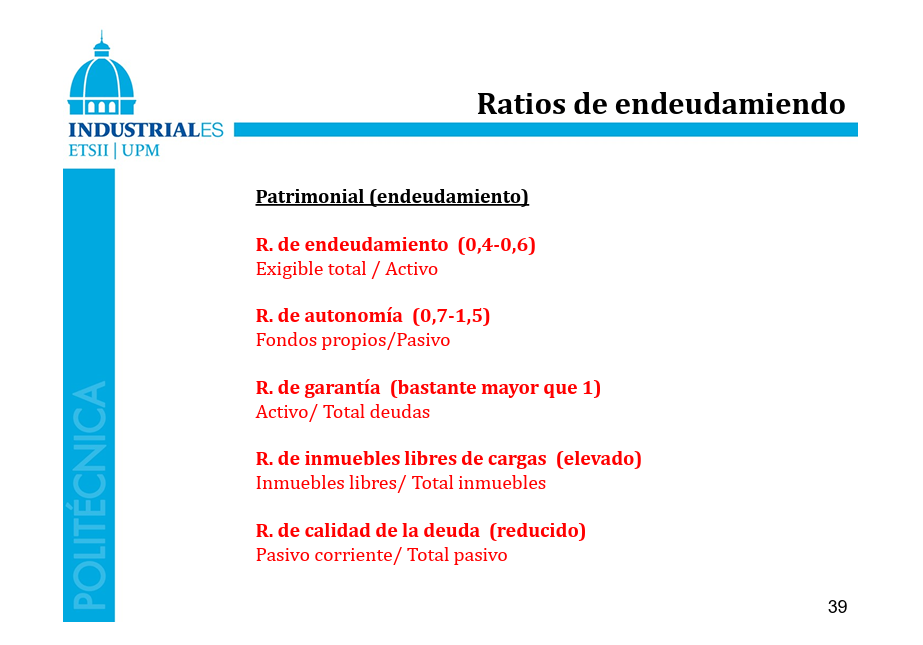
\includegraphics[width = \linewidth]{Imagenes/Ratios de endeudamiento (1).png}
    \caption{Ratios de endeudamiento}
    \label{fig:ratios de endeudamiento}
\end{figure}

\begin{figure}[h]
    \centering
    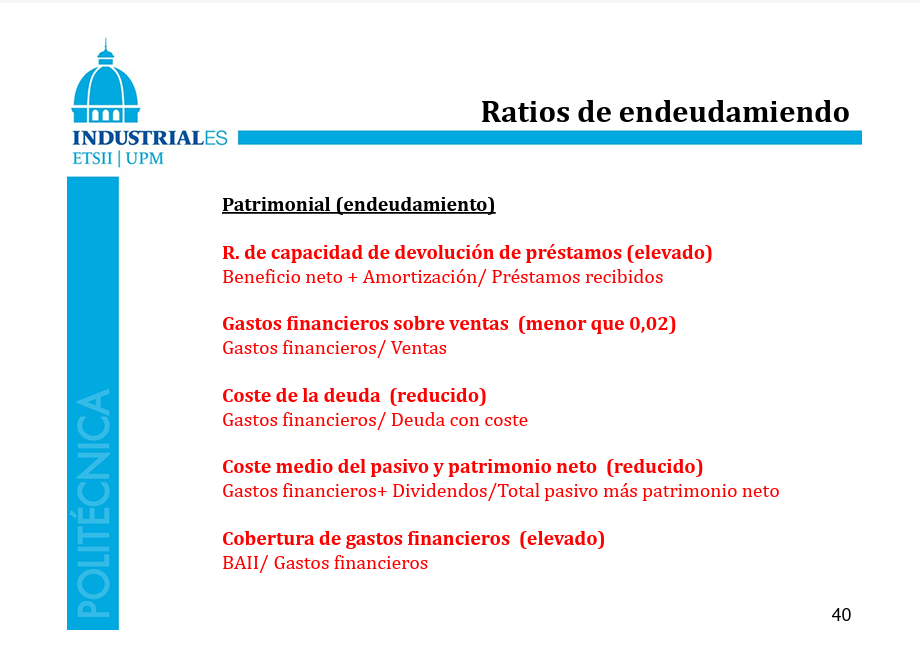
\includegraphics[width = \linewidth]{Imagenes/Ratios de endeudamiento (2).png}
    \caption{Ratios de endeudamiento (2)}
    \label{fig:ratios de endeudamiento (2)}
\end{figure}
